\documentclass{article}
\usepackage[utf8]{inputenc}
\usepackage[top=1in, bottom=1in, left=1in, right=1in]{geometry}
% \usepackage{indentfirst}
\usepackage{amsmath}
\usepackage{amssymb}
\usepackage{mathtools}
\usepackage{graphicx}
    \DeclareGraphicsExtensions{.png, .jpeg}
\usepackage{caption}
\usepackage{wrapfig}

% custom macros
\newcommand*{\doublebar}[1]{\overline{\overline{#1}}}
\newcommand*{\unknown}[0]{\;?\;}
\DeclareMathOperator*{\argmax}{argmax}

% main document
\title{MATH 786: Cooperative Game Theory \\ HW06}
\author{Terence Henriod}
\date{\today}

\begin{document}

\maketitle

\begin{abstract}
Marriage Game, Hasse Diagram, NTU Games. 
\end{abstract}

\newpage
\begin{enumerate}
\item Consider the marriage game below: \\
\begin{tabular}{ c c c }
$M_{1}$: $W_{2}$, $W_{3}$, $W_{5}$, $W_{1}$,    s.s., $W_{4}$, $W_{6}$, $W_{7}$ & \qquad
& $W_{1}$: $M_{1}$, $M_{3}$, $M_{2}$, $M_{4}$,    s.s., $M_{5}$, $M_{6}$ \\

$M_{2}$: $W_{2}$, $W_{6}$, $W_{7}$, $W_{3}$,    s.s., $W_{1}$, $W_{4}$, $W_{5}$ & \qquad
& $W_{2}$: $M_{2}$, $M_{3}$, $M_{6}$, $M_{5}$, $M_{4}$, $M_{1}$,    s.s. \\

$M_{3}$: $W_{2}$, $W_{3}$, $W_{1}$, $W_{4}$, $W_{5}$,    s.s., $W_{6}$, $W_{7}$ & \qquad
& $W_{3}$: $M_{2}$, $M_{5}$, $M_{4}$, $M_{1}$, $W_{3}$,    s.s., $M_{6}$ \\

$M_{4}$: $W_{5}$, $W_{1}$, $W_{3}$, $W_{4}$, $W_{2}$,    s.s., $W_{6}$, $W_{7}$ & \qquad
& $W_{4}$: $M_{3}$, $M_{2}$, $M_{1}$, $M_{6}$, $W_{4}$,    s.s., $M_{5}$ \\

$M_{5}$: $W_{6}$, $W_{7}$, $W_{4}$, $W_{2}$, $W_{1}$,    s.s., $W_{3}$, $W_{5}$ & \qquad
& $W_{5}$: $M_{1}$, $M_{2}$, $M_{3}$, $M_{4}$, $M_{5}$, $M_{6}$,    s.s. \\

$M_{6}$: $W_{7}$, $W_{6}$, $W_{2}$, $W_{1}$, $W_{3}$,    s.s., $W_{4}$, $W_{5}$ & \qquad
& $W_{6}$: $M_{6}$, $M_{2}$, $M_{3}$, $M_{1}$, $M_{4}$, $M_{5}$,    s.s. \\

 & \qquad
& $W_{7}$: $M_{5}$, $M_{4}$, $M_{1}$, $M_{3}$, $M_{2}$, $M_{6}$,    s.s. \\
\end{tabular}

  \begin{enumerate}
  \item Find $\mu_{m}$ and $\mu_{w}$ for this game. \\

  \textit{Solution}: \\
  $\mu_{m} = \\ \{ (M_{1} \rightarrow W_{3}),
                (M_{2} \rightarrow W_{2}),
                (M_{3} \rightarrow W_{1}),
                (M_{4} \rightarrow W_{5}),
                (M_{5} \rightarrow W_{6}),
                (M_{6} \rightarrow W_{7}),
                (\text{S.S.} \rightarrow W_{4}) \}$ \\

  $\mu_{w} = \\ \{ (W_{1} \rightarrow M_{3}),
                (W_{2} \rightarrow M_{2}),
                (W_{3} \rightarrow M_{4}),
                (W_{4} \rightarrow \text{S.S.}),
                (W_{5} \rightarrow M_{1}),
                (W_{6} \rightarrow M_{6}),
                (W_{7} \rightarrow M_{5}) \}$ \\

  The Deferred Acceptance Procedure proceeds as follows when run with the men proposing: \\

  \begin{tabular}{| l l l l l l l l |}
  \hline
  $M_{1}: R$  & $M_{2}: R$  & $M_{3}: R$  &  $M_{4}: R$ & $M_{5}: R$  & $M_{6}: R$  &             & \\
  $W_{1}: SS$ & $W_{2}: SS$ & $W_{3}: SS$ & $W_{4}: SS$ & $W_{5}: SS$ & $W_{6}: SS$ & $W_{7}: SS$ & \\
  \hline
  $M_{1}:$    & \multicolumn{7}{ l }{ propose $\rightarrow W_{2}$ } \\
              & \multicolumn{7}{ l }{ $W_{2}$ tentatively accepts; rejects S.S. } \\
  $M_{2}:$    & \multicolumn{7}{ l }{ propose $\rightarrow W_{2}$ } \\
              & \multicolumn{7}{ l }{ $W_{2}$ tentatively accepts; rejects $M_{1}$ } \\
  $M_{3}:$    & \multicolumn{7}{ l }{ propose $\rightarrow W_{2}$ } \\
              & \multicolumn{7}{ l }{ $W_{2}$ rejects } \\
  $M_{4}:$    & \multicolumn{7}{ l }{ propose $\rightarrow W_{5}$ } \\
              & \multicolumn{7}{ l }{ $W_{5}$ tentatively accepts; rejects S.S. } \\
  $M_{5}:$    & \multicolumn{7}{ l }{ propose $\rightarrow W_{6}$ } \\
              & \multicolumn{7}{ l }{ $W_{6}$ tentatively accepts; rejects S.S. } \\
  $M_{6}:$    & \multicolumn{7}{ l }{ propose $\rightarrow W_{7}$ } \\
              & \multicolumn{7}{ l }{ $W_{7}$ tentatively accepts; rejects S.S. } \\
  \hline
  $M_{1}: R$  & $M_{2}: W_{2}$  & $M_{3}: R$  &  $M_{4}: W_{5}$ & $M_{5}: W_{6}$  & $M_{6}: W_{7}$  &             & \\
  $W_{1}: SS$ & $W_{2}: M_{2}$ & $W_{3}: SS$ & $W_{4}: SS$ & $W_{5}: M_{4}$ & $W_{6}: M_{5}$ & $W_{7}: M_{6}$ & \\
  \hline
  $M_{1}:$    & \multicolumn{7}{ l }{ propose $\rightarrow W_{3}$ } \\
              & \multicolumn{7}{ l }{ $W_{3}$ tentatively accepts; rejects S.S. } \\
  $M_{2}:$    & \multicolumn{7}{ l }{ (tentatively accepted) } \\
  $M_{3}:$    & \multicolumn{7}{ l }{ propose $\rightarrow W_{3}$ } \\
              & \multicolumn{7}{ l }{ $W_{3}$ rejects } \\
  $M_{4}:$    & \multicolumn{7}{ l }{ (tentatively accepted) } \\
  $M_{5}:$    & \multicolumn{7}{ l }{ (tentatively accepted) } \\
  $M_{6}:$    & \multicolumn{7}{ l }{ (tentatively accepted) } \\
  \hline
  $M_{1}: W_{3}$  & $M_{2}: W_{2}$  & $M_{3}: R$  &  $M_{4}: W_{5}$ & $M_{5}: W_{6}$  & $M_{6}: W_{7}$  &             & \\
  $W_{1}: SS$ & $W_{2}: M_{2}$ & $W_{3}: M_{1}$ & $W_{4}: SS$ & $W_{5}: M_{4}$ & $W_{6}: M_{5}$ & $W_{7}: M_{6}$ & \\
  \hline
  $M_{1}:$    & \multicolumn{7}{ l }{ (tentatively accepted) } \\
  $M_{2}:$    & \multicolumn{7}{ l }{ (tentatively accepted) } \\
  $M_{3}:$    & \multicolumn{7}{ l }{ propose $\rightarrow W_{1}$ } \\
              & \multicolumn{7}{ l }{ $W_{1}$ tentatively accepts; rejects S.S. } \\
  $M_{4}:$    & \multicolumn{7}{ l }{ (tentatively accepted) } \\
  $M_{5}:$    & \multicolumn{7}{ l }{ (tentatively accepted) } \\
  $M_{6}:$    & \multicolumn{7}{ l }{ (tentatively accepted) } \\
  \hline
  $M_{1}: W_{3}$ & $M_{2}: W_{2}$ & $M_{3}: W_{1}$ & $M_{4}: W_{5}$ & $M_{5}: W_{6}$ & $M_{6}: W_{7}$ &                & \\
  $W_{1}: M_{4}$ & $W_{2}: M_{2}$ & $W_{3}: M_{1}$ & $W_{4}: SS$    & $W_{5}: M_{4}$ & $W_{6}: M_{5}$ & $W_{7}: M_{6}$ & \\
  \hline
  \end{tabular} \\

  ...and as follows with the women proposing: \\

  \begin{tabular}{| l l l l l l l l |}
  \hline
  $W_{1}: R$     & $W_{2}: R$     & $W_{3}: R$     & $W_{4}: R$     & $W_{5}: R$     & $W_{6}: R$     & $W_{7}: R$     & \\
  $M_{1}: SS$    & $M_{2}: SS$    & $M_{3}: SS$    &  $M_{4}: SS$   & $M_{5}: SS$    & $M_{6}: SS$     &                & \\
  \hline
  $W_{1}:$    & \multicolumn{7}{ l }{ propose $\rightarrow M_{1}$ } \\
              & \multicolumn{7}{ l }{ $M_{1}$ tentatively accepts; rejects S.S. } \\
  $W_{2}:$    & \multicolumn{7}{ l }{ propose $\rightarrow M_{2}$ } \\
              & \multicolumn{7}{ l }{ $M_{2}$ tentatively accepts; rejects S.S } \\
  $W_{3}:$    & \multicolumn{7}{ l }{ propose $\rightarrow M_{2}$ } \\
              & \multicolumn{7}{ l }{ $M_{2}$ rejects } \\
  $W_{4}:$    & \multicolumn{7}{ l }{ propose $\rightarrow M_{3}$ } \\
              & \multicolumn{7}{ l }{ $M_{3}$ tentatively accepts; rejects S.S. } \\
  $W_{5}:$    & \multicolumn{7}{ l }{ propose $\rightarrow M_{1}$ } \\
              & \multicolumn{7}{ l }{ $M_{1}$ tentatively accepts; rejects $W_{1}$ } \\
  $W_{6}:$    & \multicolumn{7}{ l }{ propose $\rightarrow M_{6}$ } \\
              & \multicolumn{7}{ l }{ $M_{6}$ tentatively accepts; rejects S.S. } \\
  $W_{7}:$    & \multicolumn{7}{ l }{ propose $\rightarrow M_{5}$ } \\
              & \multicolumn{7}{ l }{ $M_{5}$ tentatively accepts; rejects S.S. } \\
  \hline
  $W_{1}: R$     & $W_{2}: W_{2}$ & $W_{3}: R$     & $W_{4}: M_{3}$ & $W_{5}: M_{1}$ & $W_{6}: W_{6}$   & $W_{7}: M_{5}$ & \\
  $M_{1}: W_{5}$ & $M_{2}: W_{2}$ & $M_{3}: W_{4}$ &  $M_{4}: SS$   & $M_{5}: W_{7}$ & $M_{6}: W_{6}$   &                & \\
  \hline
  $W_{1}:$    & \multicolumn{7}{ l }{ propose $\rightarrow M_{3}$ } \\
              & \multicolumn{7}{ l }{ $M_{3}$ tentatively accepts; rejects $M_{4}$ } \\
  $W_{2}:$    & \multicolumn{7}{ l }{ (tentatively accepted) } \\
  $W_{3}:$    & \multicolumn{7}{ l }{ propose $\rightarrow M_{5}$ } \\
              & \multicolumn{7}{ l }{ $M_{5}$ rejects } \\
  $W_{4}:$    & \multicolumn{7}{ l }{ propose $\rightarrow M_{2}$ } \\
              & \multicolumn{7}{ l }{ $M_{2}$ rejects } \\
  $W_{5}:$    & \multicolumn{7}{ l }{ (tentatively accepted) } \\
  $W_{6}:$    & \multicolumn{7}{ l }{ (tentatively accepted) } \\
  $W_{7}:$    & \multicolumn{7}{ l }{ (tentatively accepted) } \\
  \hline
  $W_{1}: M_{3}$ & $W_{2}: W_{2}$ & $W_{3}: R$     & $W_{4}: R$     & $W_{5}: M_{1}$ & $W_{6}: W_{6}$   & $W_{7}: M_{5}$ & \\
  $M_{1}: W_{5}$ & $M_{2}: W_{2}$ & $M_{3}: W_{1}$ &  $M_{4}: SS$   & $M_{5}: W_{7}$ & $M_{6}: W_{6}$   &                & \\
  \hline
  $W_{1}:$    & \multicolumn{7}{ l }{ (tentatively accepted) } \\
  $W_{2}:$    & \multicolumn{7}{ l }{ (tentatively accepted) } \\
  $W_{3}:$    & \multicolumn{7}{ l }{ propose $\rightarrow M_{4}$ } \\
              & \multicolumn{7}{ l }{ $M_{4}$ tentatively accepts; rejects S.S. } \\
  $W_{4}:$    & \multicolumn{7}{ l }{ propose $\rightarrow M_{1}$ } \\
              & \multicolumn{7}{ l }{ $M_{1}$ rejects } \\
  $W_{5}:$    & \multicolumn{7}{ l }{ (tentatively accepted) } \\
  $W_{6}:$    & \multicolumn{7}{ l }{ (tentatively accepted) } \\
  $W_{7}:$    & \multicolumn{7}{ l }{ (tentatively accepted) } \\
  \hline
  $W_{1}: M_{3}$ & $W_{2}: W_{2}$ & $W_{3}: M_{4}$ & $W_{4}: R$     & $W_{5}: M_{1}$ & $W_{6}: W_{6}$   & $W_{7}: M_{5}$ & \\
  $M_{1}: W_{5}$ & $M_{2}: W_{2}$ & $M_{3}: W_{1}$ & $M_{4}: W_{3}$ & $M_{5}: W_{7}$ & $M_{6}: W_{6}$   &                & \\
  \hline
  $W_{4}:$    & \multicolumn{7}{ l }{ propose $\rightarrow M_{6}$ } \\
              & \multicolumn{7}{ l }{ $M_{6}$ rejects } \\
  $W_{4}:$    & \multicolumn{7}{ l }{ propose $\rightarrow M_{4}$ } \\
              & \multicolumn{7}{ l }{ $M_{4}$ rejects } \\
  $W_{4}:$    & \multicolumn{7}{ l }{ propose $\rightarrow S.S.$ } \\
              & \multicolumn{7}{ l }{ SS accepts } \\
  \hline
  $W_{1}: M_{3}$ & $W_{2}: W_{2}$ & $W_{3}: M_{4}$ & $W_{4}: SS$    & $W_{5}: M_{1}$ & $W_{6}: W_{6}$   & $W_{7}: M_{5}$ & \\
  $M_{1}: W_{5}$ & $M_{2}: W_{2}$ & $M_{3}: W_{1}$ & $M_{4}: W_{3}$ & $M_{5}: W_{7}$ & $M_{6}: W_{6}$   &                & \\
  \hline
  \end{tabular} \\

  %
  \item Find two other core matchings by trial and error. \\

  \textit{Solution}: \\

  $\mu_{1} = \\ \{ (M_{1} \rightarrow W_{5}),
                (M_{2} \rightarrow W_{2}),
                (M_{3} \rightarrow W_{1}),
                (M_{4} \rightarrow W_{3}),
                (M_{5} \rightarrow W_{6}),
                (M_{6} \rightarrow W_{7}),
                (\text{S.S.} \rightarrow W_{4}) \}$ \\

  $\mu_{2} = \\ \{ (M_{1} \rightarrow W_{3}),
                (M_{2} \rightarrow W_{2}),
                (M_{3} \rightarrow W_{1}),
                (M_{4} \rightarrow W_{5}),
                (M_{5} \rightarrow W_{7}),
                (M_{6} \rightarrow W_{6}),
                (\text{S.S.} \rightarrow W_{4}) \}$ \\

  Recall that the core of a marriage game is described as the set of matchings such that
    \begin{enumerate}
    \item $\mu(i)      \succeq^{M_{i}} \text{ s.s. } \quad \forall i \in \{1, \dots, |M|\}$
    \item $\mu^{-1}(j) \succeq^{W_{j}} \text{ s.s. } \quad \forall j \in \{1, \dots, |W|\}$
    \item $\nexists \; i, j \text{ for which } W_{j} \succeq^{M_{i}} W_{\mu(i)} \text{ AND } M_{i} \succeq^{W_{j}} W_{\mu^{-1}(j)}$
    \end{enumerate}

  Both of these pairs meet the first two, the ``individual rationality", conditions, and neither has any ``eloping" pairs (the third condition). \\

  Further, we might remark that we know which pairs in the matching cannot change: those where a player was matched to staying single, and those that do not change between the man-optimal and woman-optimal matchings. Next, by examining the preference lists, we can determine a subset of preferences that are allowable for a core matching. After taking these steps, the number of matchings to try becomes relatively small. (In this example, there are only two pairs of matchings that can ``trade" their partners after this.) \\

  %
  \item Draw a Hasse diagram for your set of core matchings. \\

  \textit{Solution}: \\

  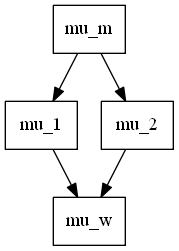
\includegraphics[scale=0.4]{hw7-1c}

  %
  \end{enumerate}
%
\item Suppose in a marriage game that $\mu_{m} = \mu_{w}$. How many core matchings must there be in this game? Justify your answer. \\

\textit{Solution}: \\

There can only be one ($1$) core matching. We know that the set of core matchings of the marriage game is a lattice, and we also know that, from the men's perspective, $\mu_{m}$ is the greatest point and $\mu_{w}$ is the least point (in the lattice sense), i.e. $\mu_{m} \ge \mu_{w}$. However, since $\mu_{m} = \mu_{w}$, for a matching to be greater than $\mu_{w}$, that point would have to also be greater than $\mu_{m}$, which, of course, is not possible if that point/matching is to still be in the core. By similar argument, there cannot be another matching that is less than $\mu_{m}$. \\

%
\item A lattice $L$ is \emph{distributive} if, for every $x, y, z \in L$, we have
\begin{align*}
\text{A) } x \wedge (y \vee z)    &=  (x \wedge y) \vee   (x \wedge z) \text{ AND} \\
\text{B) } x \vee   (y \wedge z)  &=  (x \vee y)   \wedge (x \vee z)
\end{align*}
It has been proven that the set of core matchings is always a distributive finite lattice (the converse of this statement, although it has to be more carefully stated, is also true).

In the ``ten" core matchings example from class, verify A) and B) in the case where x = $\mu_{5}$, $y = \mu_{6}$, and $z = \mu_{9}$. \\

\textit{Solution}: \\

Recall that the Hasse diagram ranks the matchings, and from it we can easily determine the $\vee$ and $\wedge$ rlationship between two matchings, where $a \vee b$ is the matching that is the lowest common element at or above $a, b$, and $a \wedge b$ is the matching that is the highest common element at or below $a, b$.

A)\begin{align*}
\mu_{5} \wedge (\mu_{6} \vee \mu_{9})    &=  (\mu_{5} \wedge \mu_{6}) \vee   (\mu_{5} \wedge \mu{9}) \\
\mu_{5} \wedge \mu_{6}                   &=  \mu_{7}                  \vee   \mu_{9} \\
\mu_{7}                                  &=  \mu_{7}  \qquad \surd
\end{align*}

B)\begin{align*}
\mu_{5} \vee   (\mu_{6} \wedge \mu_{9})  &=  (\mu_{5} \vee \mu_{6})   \wedge (\mu_{5} \vee \mu_{9}) \\
\mu_{5} \vee   \mu_{9}                   &=  \mu_{4}                  \wedge \mu_{5} \\
\mu_{5}                                  &=  \mu_{5}  \qquad \surd
\end{align*}

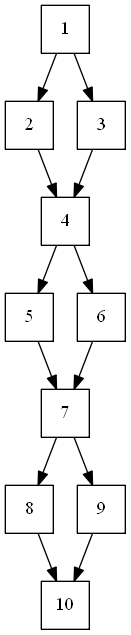
\includegraphics[width=0.07\textwidth]{hw7-3}

%
\item Suppose a given marriage game in which $|M| = |W| = m \;(m \text{ odd})$. For simplicity, also assume that every player's last choice is ``s.s.". Show that $\mu_{m}$ must give the players on average at least their $\frac{m + 1}{2}^{th}$ choice. HINT: Consider the ``total ranking" for the men under $\mu_{m}$ (by ``total ranking" we mean the sum of all the men's individual ranking fo the women they get under $\mu_{m}$), and consider the ramifications of this quantity for the DAP. \\

\textit{Solution}: \\

Start by considering a ``worst case" (or perhaps ``most extreme case") man-optimal matching, where each man gets his first choice, and each woman gets her last choice (above s.s. since she did get matched). In this case, the total ranking of the men's choices is $m$, and the total ranking of the women's choices is $m * m$. In this scenario, since there are $2m$ players, for the average player we have:
\[ \frac{m + m^{2}}{2m} = \frac{1 + m}{2} \]

Now, suppose we alter things to make the outcome less extreme. If we alter the game so that any man does worse, than at there is a woman who must do better. This is because for a man to do worse, he mst get rejected, and each time a woman rejects him, that implies that she has at least one prospect who is better that proposed to her. So even as we alter the game, we see that the net total ranking cannot decrease. This argument covers all of the cases that are less extreme than our original one.

Since we considered the most extreme case, and deviation from it, we can say that in all other cases, players will actually do better in terms of the rankings of their partners on average than $\frac{1 + m}{2}$.

%
\item Consider the modeling of NTU games in which the characteristic function values $V(S)$ are sets in $\mathbb{R}^{S}$ (and not $\mathbb{R}^{N}$). State the definition of superadditivity in this case. \\

\textit{Solution}: \\

If an NTU game is superadditive then it must satisfy $V(A) \times V(B) \subset V(A \cup B) \quad \forall \; A \in \mathbb{R}^{S_{1}}, B \in \mathbb{R}^{S_{2}}, A \cup B = \emptyset$.

Superadditivity, in any sense, means that the total value of coalitions working separately must not exceed the value of those coalitions working together. In the NTU-sense, this means that the region specified by the $V(S)$s must not be outside the regions defined by the $V(S)$ for the coalitions together. If we consider the one dimensional (one player) case for each $S_{1}, S_{2}$, then we might say that $A$ represents all of the payoffs that player $1$ can achieve (call the best one $a$), and $B$ represents the payoffs $2$ can achieve (call the best one $b$). Together, the two players can achieve any combination of payofs inside the region bounded by $(0, 0)$, $(0, b)$, $(a, 0)$, and $(a,b)$. Similar logic can be used in higher dimensions (with coalitions of more players).

%
\end{enumerate}
\end{document}
